\documentclass{standalone}
\usepackage{tikz}
\usetikzlibrary{patterns, positioning}

\begin{document}
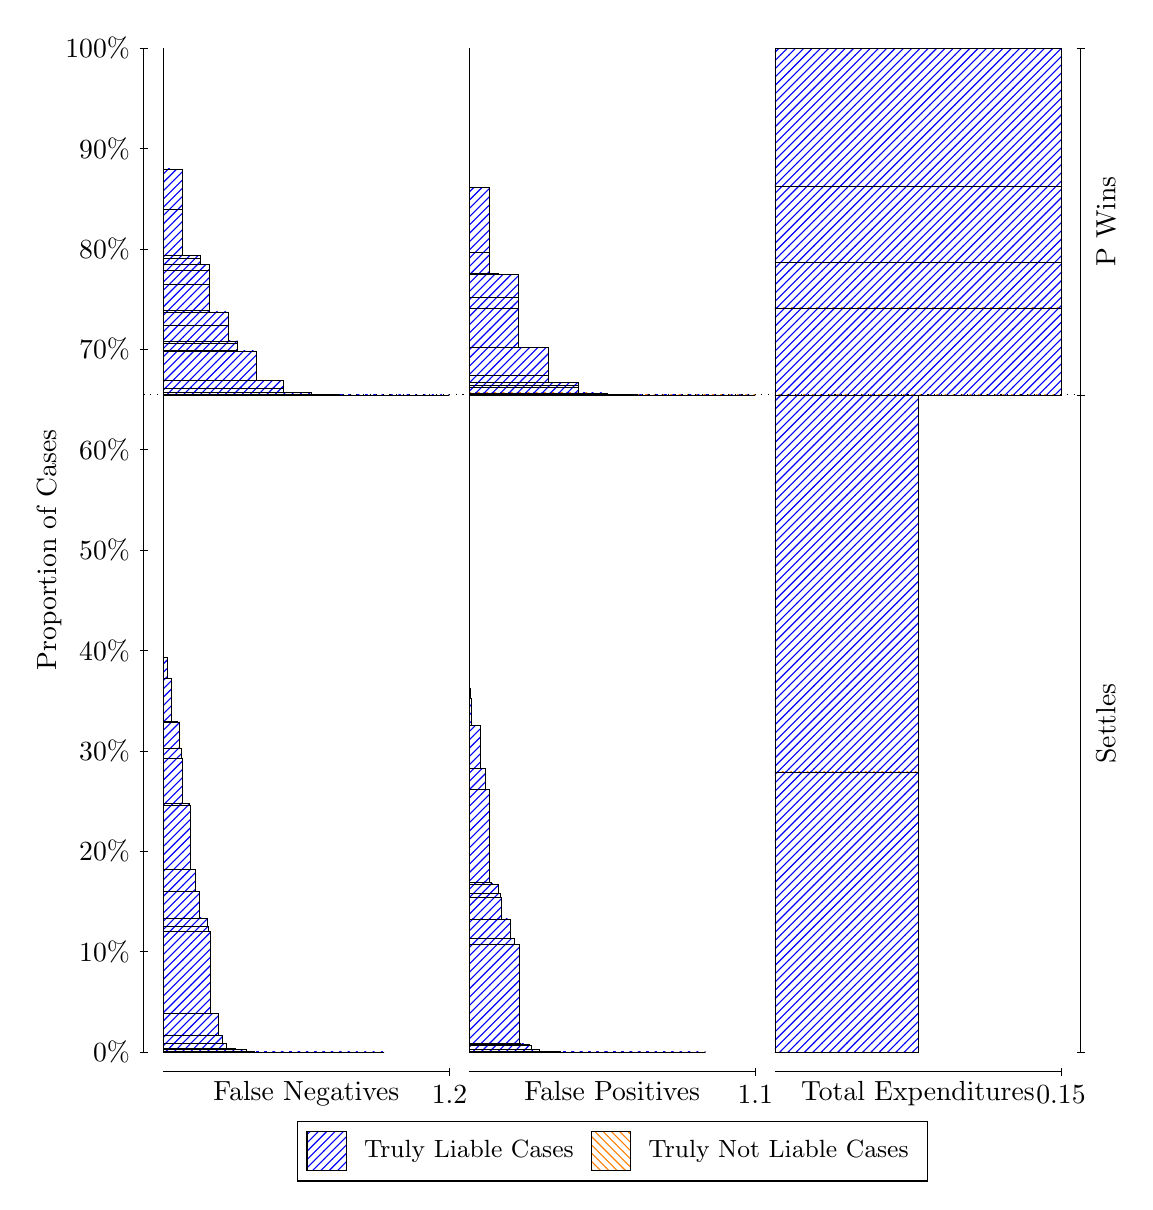
\begin{tikzpicture}
\draw[black, very thin] (1.5,1.75) -- (1.5,14.5);
\node[rotate=90, anchor=center] at (0.3, 8.125) {Proportion of Cases};
\draw[black, very thin] (1.45,1.75) -- (1.55,1.75);
\node[anchor=east] at (1.45, 1.75) {0\%};
\draw[black, very thin] (1.45,3.025) -- (1.55,3.025);
\node[anchor=east] at (1.45, 3.025) {10\%};
\draw[black, very thin] (1.45,4.3) -- (1.55,4.3);
\node[anchor=east] at (1.45, 4.3) {20\%};
\draw[black, very thin] (1.45,5.575) -- (1.55,5.575);
\node[anchor=east] at (1.45, 5.575) {30\%};
\draw[black, very thin] (1.45,6.85) -- (1.55,6.85);
\node[anchor=east] at (1.45, 6.85) {40\%};
\draw[black, very thin] (1.45,8.125) -- (1.55,8.125);
\node[anchor=east] at (1.45, 8.125) {50\%};
\draw[black, very thin] (1.45,9.4) -- (1.55,9.4);
\node[anchor=east] at (1.45, 9.4) {60\%};
\draw[black, very thin] (1.45,10.675) -- (1.55,10.675);
\node[anchor=east] at (1.45, 10.675) {70\%};
\draw[black, very thin] (1.45,11.95) -- (1.55,11.95);
\node[anchor=east] at (1.45, 11.95) {80\%};
\draw[black, very thin] (1.45,13.225) -- (1.55,13.225);
\node[anchor=east] at (1.45, 13.225) {90\%};
\draw[black, very thin] (1.45,14.5) -- (1.55,14.5);
\node[anchor=east] at (1.45, 14.5) {100\%};

\draw[black, very thin] (13.4,1.75) -- (13.4,14.5);
\draw[black, very thin] (13.35,1.75) -- (13.45,1.75);
\node[anchor=west] at (13.35, 1.75) {};
\draw[black, very thin] (13.35,10.095) -- (13.45,10.095);
\node[anchor=west] at (13.35, 10.095) {};
\draw[black, very thin] (13.35,14.5) -- (13.45,14.5);
\node[anchor=west] at (13.35, 14.5) {};

\draw[black, very thin, pattern color=blue, pattern=north east lines] (1.75,1.75) rectangle (4.554,1.75);
\draw[black, very thin, pattern color=blue, pattern=north east lines] (1.75,1.75) rectangle (4.2029,1.75);
\draw[black, very thin, pattern color=blue, pattern=north east lines] (1.75,1.75) rectangle (4.0801,1.75);
\draw[black, very thin, pattern color=blue, pattern=north east lines] (1.75,1.75) rectangle (3.8519,1.75);
\draw[black, very thin, pattern color=blue, pattern=north east lines] (1.75,1.75) rectangle (3.729,1.75);
\draw[black, very thin, pattern color=blue, pattern=north east lines] (1.75,1.75) rectangle (3.6062,1.75);
\draw[black, very thin, pattern color=blue, pattern=north east lines] (1.75,1.75) rectangle (3.5008,1.75);
\draw[black, very thin, pattern color=blue, pattern=north east lines] (1.75,1.75) rectangle (3.4482,1.75);
\draw[black, very thin, pattern color=blue, pattern=north east lines] (1.75,1.75) rectangle (3.378,1.75);
\draw[black, very thin, pattern color=blue, pattern=north east lines] (1.75,1.75) rectangle (3.2551,1.75);
\draw[black, very thin, pattern color=blue, pattern=north east lines] (1.75,1.75) rectangle (3.1498,1.7506);
\draw[black, very thin, pattern color=blue, pattern=north east lines] (1.75,1.7506) rectangle (3.1322,1.7506);
\draw[black, very thin, pattern color=blue, pattern=north east lines] (1.75,1.7506) rectangle (3.0971,1.7506);
\draw[black, very thin, pattern color=blue, pattern=north east lines] (1.75,1.7506) rectangle (3.0269,1.7508);
\draw[black, very thin, pattern color=blue, pattern=north east lines] (1.75,1.7508) rectangle (2.9743,1.7508);
\draw[black, very thin, pattern color=blue, pattern=north east lines] (1.75,1.7508) rectangle (2.9041,1.7532);
\draw[black, very thin, pattern color=blue, pattern=north east lines] (1.75,1.7532) rectangle (2.7988,1.7795);
\draw[black, very thin, pattern color=blue, pattern=north east lines] (1.75,1.7795) rectangle (2.7812,1.7796);
\draw[black, very thin, pattern color=blue, pattern=north east lines] (1.75,1.7796) rectangle (2.7461,1.7796);
\draw[black, very thin, pattern color=blue, pattern=north east lines] (1.75,1.7796) rectangle (2.6759,1.7865);
\draw[black, very thin, pattern color=blue, pattern=north east lines] (1.75,1.7865) rectangle (2.6583,1.7973);
\draw[black, very thin, pattern color=blue, pattern=north east lines] (1.75,1.7973) rectangle (2.6232,1.7975);
\draw[black, very thin, pattern color=blue, pattern=north east lines] (1.75,1.7975) rectangle (2.553,1.8557);
\draw[black, very thin, pattern color=blue, pattern=north east lines] (1.75,1.8557) rectangle (2.5004,1.967);
\draw[black, very thin, pattern color=blue, pattern=north east lines] (1.75,1.967) rectangle (2.4477,2.2389);
\draw[black, very thin, pattern color=blue, pattern=north east lines] (1.75,2.2389) rectangle (2.4302,2.2419);
\draw[black, very thin, pattern color=blue, pattern=north east lines] (1.75,2.2419) rectangle (2.395,2.242);
\draw[black, very thin, pattern color=blue, pattern=north east lines] (1.75,2.242) rectangle (2.3424,3.2825);
\draw[black, very thin, pattern color=blue, pattern=north east lines] (1.75,3.2825) rectangle (2.3248,3.3409);
\draw[black, very thin, pattern color=blue, pattern=north east lines] (1.75,3.3409) rectangle (2.3073,3.45);
\draw[black, very thin, pattern color=blue, pattern=north east lines] (1.75,3.45) rectangle (2.2722,3.4524);
\draw[black, very thin, pattern color=blue, pattern=north east lines] (1.75,3.4524) rectangle (2.202,3.7868);
\draw[black, very thin, pattern color=blue, pattern=north east lines] (1.75,3.7868) rectangle (2.1493,4.0688);
\draw[black, very thin, pattern color=blue, pattern=north east lines] (1.75,4.0688) rectangle (2.0967,4.8889);
\draw[black, very thin, pattern color=blue, pattern=north east lines] (1.75,4.8889) rectangle (2.0791,4.9094);
\draw[black, very thin, pattern color=blue, pattern=north east lines] (1.75,4.9094) rectangle (2.044,4.9094);
\draw[black, very thin, pattern color=blue, pattern=north east lines] (1.75,4.9094) rectangle (1.9913,5.4807);
\draw[black, very thin, pattern color=blue, pattern=north east lines] (1.75,5.4807) rectangle (1.9738,5.602);
\draw[black, very thin, pattern color=blue, pattern=north east lines] (1.75,5.602) rectangle (1.9562,5.9407);
\draw[black, very thin, pattern color=blue, pattern=north east lines] (1.75,5.9407) rectangle (1.9211,5.9464);
\draw[black, very thin, pattern color=blue, pattern=north east lines] (1.75,5.9464) rectangle (1.8509,6.4927);
\draw[black, very thin, pattern color=blue, pattern=north east lines] (1.75,6.4927) rectangle (1.7983,6.7601);
\draw[black, very thin, pattern color=orange, pattern=north west lines] (1.75,6.7601) rectangle (1.75,6.7601);
\draw[black, very thin, pattern color=blue, pattern=north east lines] (1.75,6.7601) rectangle (1.75,10.095);
\draw[black, very thin, pattern color=blue, pattern=north east lines] (1.75,10.095) rectangle (5.3833,10.095);
\draw[black, very thin, pattern color=blue, pattern=north east lines] (1.75,10.095) rectangle (5.0323,10.095);
\draw[black, very thin, pattern color=blue, pattern=north east lines] (1.75,10.095) rectangle (5.0323,10.095);
\draw[black, very thin, pattern color=blue, pattern=north east lines] (1.75,10.095) rectangle (4.6812,10.095);
\draw[black, very thin, pattern color=blue, pattern=north east lines] (1.75,10.095) rectangle (4.6812,10.095);
\draw[black, very thin, pattern color=blue, pattern=north east lines] (1.75,10.095) rectangle (4.4443,10.095);
\draw[black, very thin, pattern color=blue, pattern=north east lines] (1.75,10.095) rectangle (4.3302,10.095);
\draw[black, very thin, pattern color=blue, pattern=north east lines] (1.75,10.095) rectangle (4.0932,10.095);
\draw[black, very thin, pattern color=blue, pattern=north east lines] (1.75,10.095) rectangle (3.9791,10.097);
\draw[black, very thin, pattern color=blue, pattern=north east lines] (1.75,10.097) rectangle (3.9791,10.099);
\draw[black, very thin, pattern color=blue, pattern=north east lines] (1.75,10.099) rectangle (3.7422,10.099);
\draw[black, very thin, pattern color=blue, pattern=north east lines] (1.75,10.099) rectangle (3.6281,10.128);
\draw[black, very thin, pattern color=blue, pattern=north east lines] (1.75,10.128) rectangle (3.3911,10.128);
\draw[black, very thin, pattern color=blue, pattern=north east lines] (1.75,10.128) rectangle (3.3911,10.128);
\draw[black, very thin, pattern color=blue, pattern=north east lines] (1.75,10.128) rectangle (3.2771,10.185);
\draw[black, very thin, pattern color=blue, pattern=north east lines] (1.75,10.185) rectangle (3.2771,10.275);
\draw[black, very thin, pattern color=blue, pattern=north east lines] (1.75,10.275) rectangle (3.0401,10.279);
\draw[black, very thin, pattern color=blue, pattern=north east lines] (1.75,10.279) rectangle (3.0401,10.28);
\draw[black, very thin, pattern color=blue, pattern=north east lines] (1.75,10.28) rectangle (3.0401,10.284);
\draw[black, very thin, pattern color=blue, pattern=north east lines] (1.75,10.284) rectangle (2.926,10.653);
\draw[black, very thin, pattern color=blue, pattern=north east lines] (1.75,10.653) rectangle (2.689,10.662);
\draw[black, very thin, pattern color=blue, pattern=north east lines] (1.75,10.662) rectangle (2.689,10.75);
\draw[black, very thin, pattern color=blue, pattern=north east lines] (1.75,10.75) rectangle (2.689,10.782);
\draw[black, very thin, pattern color=blue, pattern=north east lines] (1.75,10.782) rectangle (2.575,10.976);
\draw[black, very thin, pattern color=blue, pattern=north east lines] (1.75,10.976) rectangle (2.575,11.148);
\draw[black, very thin, pattern color=blue, pattern=north east lines] (1.75,11.148) rectangle (2.338,11.165);
\draw[black, very thin, pattern color=blue, pattern=north east lines] (1.75,11.165) rectangle (2.338,11.497);
\draw[black, very thin, pattern color=blue, pattern=north east lines] (1.75,11.497) rectangle (2.338,11.673);
\draw[black, very thin, pattern color=blue, pattern=north east lines] (1.75,11.673) rectangle (2.338,11.751);
\draw[black, very thin, pattern color=blue, pattern=north east lines] (1.75,11.751) rectangle (2.2239,11.827);
\draw[black, very thin, pattern color=blue, pattern=north east lines] (1.75,11.827) rectangle (2.2239,11.867);
\draw[black, very thin, pattern color=blue, pattern=north east lines] (1.75,11.867) rectangle (1.987,12.447);
\draw[black, very thin, pattern color=blue, pattern=north east lines] (1.75,12.447) rectangle (1.987,12.956);
\draw[black, very thin, pattern color=blue, pattern=north east lines] (1.75,12.956) rectangle (1.8729,12.956);
\draw[black, very thin, pattern color=blue, pattern=north east lines] (1.75,12.956) rectangle (1.8729,12.962);
\draw[black, very thin, pattern color=blue, pattern=north east lines] (1.75,12.962) rectangle (1.8729,12.966);
\draw[black, very thin, pattern color=blue, pattern=north east lines] (1.75,12.966) rectangle (1.8729,12.966);
\draw[black, very thin, pattern color=orange, pattern=north west lines] (1.75,12.966) rectangle (1.75,12.966);
\draw[black, very thin, pattern color=blue, pattern=north east lines] (1.75,12.966) rectangle (1.75,14.5);
\draw[black, very thin, pattern color=orange, pattern=north west lines] (5.6333,1.75) rectangle (8.6329,1.75);
\draw[black, very thin, pattern color=blue, pattern=north east lines] (5.6333,1.75) rectangle (8.6329,1.75);
\draw[black, very thin, pattern color=orange, pattern=north west lines] (5.6333,1.75) rectangle (8.464,1.75);
\draw[black, very thin, pattern color=blue, pattern=north east lines] (5.6333,1.75) rectangle (8.464,1.75);
\draw[black, very thin, pattern color=orange, pattern=north west lines] (5.6333,1.75) rectangle (8.295,1.75);
\draw[black, very thin, pattern color=blue, pattern=north east lines] (5.6333,1.75) rectangle (8.295,1.75);
\draw[black, very thin, pattern color=blue, pattern=north east lines] (5.6333,1.75) rectangle (8.2574,1.75);
\draw[black, very thin, pattern color=blue, pattern=north east lines] (5.6333,1.75) rectangle (8.0884,1.75);
\draw[black, very thin, pattern color=orange, pattern=north west lines] (5.6333,1.75) rectangle (7.957,1.75);
\draw[black, very thin, pattern color=blue, pattern=north east lines] (5.6333,1.75) rectangle (7.957,1.75);
\draw[black, very thin, pattern color=blue, pattern=north east lines] (5.6333,1.75) rectangle (7.9194,1.75);
\draw[black, very thin, pattern color=blue, pattern=north east lines] (5.6333,1.75) rectangle (7.8819,1.75);
\draw[black, very thin, pattern color=orange, pattern=north west lines] (5.6333,1.75) rectangle (7.788,1.75);
\draw[black, very thin, pattern color=blue, pattern=north east lines] (5.6333,1.75) rectangle (7.788,1.75);
\draw[black, very thin, pattern color=blue, pattern=north east lines] (5.6333,1.75) rectangle (7.7129,1.75);
\draw[black, very thin, pattern color=blue, pattern=north east lines] (5.6333,1.75) rectangle (7.5814,1.75);
\draw[black, very thin, pattern color=blue, pattern=north east lines] (5.6333,1.75) rectangle (7.5439,1.75);
\draw[black, very thin, pattern color=blue, pattern=north east lines] (5.6333,1.75) rectangle (7.5063,1.75);
\draw[black, very thin, pattern color=orange, pattern=north west lines] (5.6333,1.75) rectangle (7.45,1.75);
\draw[black, very thin, pattern color=blue, pattern=north east lines] (5.6333,1.75) rectangle (7.45,1.75);
\draw[black, very thin, pattern color=blue, pattern=north east lines] (5.6333,1.75) rectangle (7.4124,1.75);
\draw[black, very thin, pattern color=blue, pattern=north east lines] (5.6333,1.75) rectangle (7.3373,1.75);
\draw[black, very thin, pattern color=orange, pattern=north west lines] (5.6333,1.75) rectangle (7.281,1.75);
\draw[black, very thin, pattern color=blue, pattern=north east lines] (5.6333,1.75) rectangle (7.281,1.75);
\draw[black, very thin, pattern color=blue, pattern=north east lines] (5.6333,1.75) rectangle (7.2059,1.75);
\draw[black, very thin, pattern color=blue, pattern=north east lines] (5.6333,1.75) rectangle (7.1683,1.75);
\draw[black, very thin, pattern color=blue, pattern=north east lines] (5.6333,1.75) rectangle (7.1308,1.75);
\draw[black, very thin, pattern color=blue, pattern=north east lines] (5.6333,1.75) rectangle (7.0745,1.75);
\draw[black, very thin, pattern color=blue, pattern=north east lines] (5.6333,1.75) rectangle (7.0369,1.75);
\draw[black, very thin, pattern color=blue, pattern=north east lines] (5.6333,1.75) rectangle (6.9618,1.7501);
\draw[black, very thin, pattern color=blue, pattern=north east lines] (5.6333,1.7501) rectangle (6.9055,1.7507);
\draw[black, very thin, pattern color=blue, pattern=north east lines] (5.6333,1.7507) rectangle (6.8304,1.7507);
\draw[black, very thin, pattern color=blue, pattern=north east lines] (5.6333,1.7507) rectangle (6.7928,1.7531);
\draw[black, very thin, pattern color=orange, pattern=north west lines] (5.6333,1.7531) rectangle (6.774,1.7531);
\draw[black, very thin, pattern color=blue, pattern=north east lines] (5.6333,1.7531) rectangle (6.774,1.7535);
\draw[black, very thin, pattern color=blue, pattern=north east lines] (5.6333,1.7535) rectangle (6.7553,1.7535);
\draw[black, very thin, pattern color=blue, pattern=north east lines] (5.6333,1.7535) rectangle (6.6989,1.7535);
\draw[black, very thin, pattern color=blue, pattern=north east lines] (5.6333,1.7535) rectangle (6.6614,1.7537);
\draw[black, very thin, pattern color=blue, pattern=north east lines] (5.6333,1.7537) rectangle (6.5863,1.7592);
\draw[black, very thin, pattern color=blue, pattern=north east lines] (5.6333,1.7592) rectangle (6.5299,1.7852);
\draw[black, very thin, pattern color=blue, pattern=north east lines] (5.6333,1.7852) rectangle (6.4548,1.7854);
\draw[black, very thin, pattern color=blue, pattern=north east lines] (5.6333,1.7854) rectangle (6.4173,1.8384);
\draw[black, very thin, pattern color=blue, pattern=north east lines] (5.6333,1.8384) rectangle (6.3985,1.8462);
\draw[black, very thin, pattern color=blue, pattern=north east lines] (5.6333,1.8462) rectangle (6.3797,1.8519);
\draw[black, very thin, pattern color=blue, pattern=north east lines] (5.6333,1.8519) rectangle (6.3234,1.8519);
\draw[black, very thin, pattern color=blue, pattern=north east lines] (5.6333,1.8519) rectangle (6.2858,1.8567);
\draw[black, very thin, pattern color=orange, pattern=north west lines] (5.6333,1.8567) rectangle (6.2671,1.8567);
\draw[black, very thin, pattern color=blue, pattern=north east lines] (5.6333,1.8567) rectangle (6.2671,3.1198);
\draw[black, very thin, pattern color=blue, pattern=north east lines] (5.6333,3.1198) rectangle (6.2107,3.1933);
\draw[black, very thin, pattern color=blue, pattern=north east lines] (5.6333,3.1933) rectangle (6.1544,3.4391);
\draw[black, very thin, pattern color=blue, pattern=north east lines] (5.6333,3.4391) rectangle (6.0793,3.4415);
\draw[black, very thin, pattern color=blue, pattern=north east lines] (5.6333,3.4415) rectangle (6.0417,3.7086);
\draw[black, very thin, pattern color=blue, pattern=north east lines] (5.6333,3.7086) rectangle (6.023,3.7677);
\draw[black, very thin, pattern color=blue, pattern=north east lines] (5.6333,3.7677) rectangle (6.0042,3.8857);
\draw[black, very thin, pattern color=blue, pattern=north east lines] (5.6333,3.8857) rectangle (5.9478,3.8858);
\draw[black, very thin, pattern color=blue, pattern=north east lines] (5.6333,3.8858) rectangle (5.9103,3.9091);
\draw[black, very thin, pattern color=blue, pattern=north east lines] (5.6333,3.9091) rectangle (5.8915,5.085);
\draw[black, very thin, pattern color=blue, pattern=north east lines] (5.6333,5.085) rectangle (5.8352,5.3524);
\draw[black, very thin, pattern color=blue, pattern=north east lines] (5.6333,5.3524) rectangle (5.7789,5.8987);
\draw[black, very thin, pattern color=blue, pattern=north east lines] (5.6333,5.8987) rectangle (5.7037,5.9043);
\draw[black, very thin, pattern color=blue, pattern=north east lines] (5.6333,5.9043) rectangle (5.6662,6.2431);
\draw[black, very thin, pattern color=blue, pattern=north east lines] (5.6333,6.2431) rectangle (5.6474,6.3643);
\draw[black, very thin, pattern color=blue, pattern=north east lines] (5.6333,6.3643) rectangle (5.6333,10.095);
\draw[black, very thin, pattern color=orange, pattern=north west lines] (5.6333,10.095) rectangle (9.2667,10.095);
\draw[black, very thin, pattern color=blue, pattern=north east lines] (5.6333,10.095) rectangle (9.2667,10.095);
\draw[black, very thin, pattern color=orange, pattern=north west lines] (5.6333,10.095) rectangle (8.8911,10.095);
\draw[black, very thin, pattern color=blue, pattern=north east lines] (5.6333,10.095) rectangle (8.8911,10.095);
\draw[black, very thin, pattern color=orange, pattern=north west lines] (5.6333,10.095) rectangle (8.5156,10.095);
\draw[black, very thin, pattern color=blue, pattern=north east lines] (5.6333,10.095) rectangle (8.5156,10.095);
\draw[black, very thin, pattern color=blue, pattern=north east lines] (5.6333,10.095) rectangle (8.5156,10.095);
\draw[black, very thin, pattern color=blue, pattern=north east lines] (5.6333,10.095) rectangle (8.1401,10.095);
\draw[black, very thin, pattern color=orange, pattern=north west lines] (5.6333,10.095) rectangle (8.1401,10.095);
\draw[black, very thin, pattern color=blue, pattern=north east lines] (5.6333,10.095) rectangle (8.1401,10.095);
\draw[black, very thin, pattern color=orange, pattern=north west lines] (5.6333,10.095) rectangle (7.8866,10.095);
\draw[black, very thin, pattern color=blue, pattern=north east lines] (5.6333,10.095) rectangle (7.8866,10.095);
\draw[black, very thin, pattern color=orange, pattern=north west lines] (5.6333,10.095) rectangle (7.7645,10.095);
\draw[black, very thin, pattern color=blue, pattern=north east lines] (5.6333,10.095) rectangle (7.7645,10.097);
\draw[black, very thin, pattern color=orange, pattern=north west lines] (5.6333,10.097) rectangle (7.511,10.097);
\draw[black, very thin, pattern color=blue, pattern=north east lines] (5.6333,10.097) rectangle (7.511,10.097);
\draw[black, very thin, pattern color=orange, pattern=north west lines] (5.6333,10.097) rectangle (7.389,10.097);
\draw[black, very thin, pattern color=blue, pattern=north east lines] (5.6333,10.097) rectangle (7.389,10.12);
\draw[black, very thin, pattern color=blue, pattern=north east lines] (5.6333,10.12) rectangle (7.1355,10.12);
\draw[black, very thin, pattern color=orange, pattern=north west lines] (5.6333,10.12) rectangle (7.1355,10.12);
\draw[black, very thin, pattern color=blue, pattern=north east lines] (5.6333,10.12) rectangle (7.1355,10.12);
\draw[black, very thin, pattern color=orange, pattern=north west lines] (5.6333,10.12) rectangle (7.0134,10.12);
\draw[black, very thin, pattern color=blue, pattern=north east lines] (5.6333,10.12) rectangle (7.0134,10.192);
\draw[black, very thin, pattern color=blue, pattern=north east lines] (5.6333,10.192) rectangle (7.0134,10.22);
\draw[black, very thin, pattern color=blue, pattern=north east lines] (5.6333,10.22) rectangle (7.0134,10.253);
\draw[black, very thin, pattern color=blue, pattern=north east lines] (5.6333,10.253) rectangle (6.7599,10.253);
\draw[black, very thin, pattern color=orange, pattern=north west lines] (5.6333,10.253) rectangle (6.7599,10.253);
\draw[black, very thin, pattern color=blue, pattern=north east lines] (5.6333,10.253) rectangle (6.7599,10.253);
\draw[black, very thin, pattern color=orange, pattern=north west lines] (5.6333,10.253) rectangle (6.6379,10.253);
\draw[black, very thin, pattern color=blue, pattern=north east lines] (5.6333,10.253) rectangle (6.6379,10.338);
\draw[black, very thin, pattern color=blue, pattern=north east lines] (5.6333,10.338) rectangle (6.6379,10.703);
\draw[black, very thin, pattern color=blue, pattern=north east lines] (5.6333,10.703) rectangle (6.3844,10.703);
\draw[black, very thin, pattern color=orange, pattern=north west lines] (5.6333,10.703) rectangle (6.3844,10.703);
\draw[black, very thin, pattern color=blue, pattern=north east lines] (5.6333,10.703) rectangle (6.3844,10.703);
\draw[black, very thin, pattern color=blue, pattern=north east lines] (5.6333,10.703) rectangle (6.2624,11.2);
\draw[black, very thin, pattern color=blue, pattern=north east lines] (5.6333,11.2) rectangle (6.2624,11.33);
\draw[black, very thin, pattern color=blue, pattern=north east lines] (5.6333,11.33) rectangle (6.2624,11.629);
\draw[black, very thin, pattern color=blue, pattern=north east lines] (5.6333,11.629) rectangle (6.0089,11.629);
\draw[black, very thin, pattern color=orange, pattern=north west lines] (5.6333,11.629) rectangle (6.0089,11.629);
\draw[black, very thin, pattern color=blue, pattern=north east lines] (5.6333,11.629) rectangle (6.0089,11.639);
\draw[black, very thin, pattern color=blue, pattern=north east lines] (5.6333,11.639) rectangle (6.0089,11.639);
\draw[black, very thin, pattern color=blue, pattern=north east lines] (5.6333,11.639) rectangle (5.8868,11.901);
\draw[black, very thin, pattern color=blue, pattern=north east lines] (5.6333,11.901) rectangle (5.8868,12.728);
\draw[black, very thin, pattern color=orange, pattern=north west lines] (5.6333,12.728) rectangle (5.6333,12.728);
\draw[black, very thin, pattern color=blue, pattern=north east lines] (5.6333,12.728) rectangle (5.6333,14.5);
\draw[black, very thin, pattern color=orange, pattern=north west lines] (9.5167,1.75) rectangle (11.333,1.75);
\draw[black, very thin, pattern color=blue, pattern=north east lines] (9.5167,1.75) rectangle (11.333,5.3077);
\draw[black, very thin, pattern color=orange, pattern=north west lines] (9.5167,5.3077) rectangle (11.333,5.3077);
\draw[black, very thin, pattern color=blue, pattern=north east lines] (9.5167,5.3077) rectangle (11.333,10.095);
\draw[black, very thin, pattern color=orange, pattern=north west lines] (9.5167,10.095) rectangle (13.15,10.095);
\draw[black, very thin, pattern color=blue, pattern=north east lines] (9.5167,10.095) rectangle (13.15,11.2);
\draw[black, very thin, pattern color=orange, pattern=north west lines] (9.5167,11.2) rectangle (13.15,11.2);
\draw[black, very thin, pattern color=blue, pattern=north east lines] (9.5167,11.2) rectangle (13.15,11.778);
\draw[black, very thin, pattern color=orange, pattern=north west lines] (9.5167,11.778) rectangle (13.15,11.778);
\draw[black, very thin, pattern color=blue, pattern=north east lines] (9.5167,11.778) rectangle (13.15,12.738);
\draw[black, very thin, pattern color=orange, pattern=north west lines] (9.5167,12.738) rectangle (13.15,12.738);
\draw[black, very thin, pattern color=blue, pattern=north east lines] (9.5167,12.738) rectangle (13.15,14.5);
\draw[black, dotted] (1.5,10.095) -- (13.4,10.095);
\draw[black, very thin] (1.75,1.5) -- (5.3833,1.5);
\node[anchor=north] at (3.5667, 1.5) {False Negatives};
\draw[black, very thin] (5.3833,1.45) -- (5.3833,1.55);
\node[anchor=north] at (5.3833, 1.45) {1.2};

\draw[black, very thin] (5.6333,1.5) -- (9.2667,1.5);
\node[anchor=north] at (7.45, 1.5) {False Positives};
\draw[black, very thin] (9.2667,1.45) -- (9.2667,1.55);
\node[anchor=north] at (9.2667, 1.45) {1.1};

\draw[black, very thin] (9.5167,1.5) -- (13.15,1.5);
\node[anchor=north] at (11.333, 1.5) {Total Expenditures};
\draw[black, very thin] (13.15,1.45) -- (13.15,1.55);
\node[anchor=north] at (13.15, 1.45) {0.15};

\node[black, centered, rotate=90] at (13.72, 5.9225) {Settles};
\node[black, centered, rotate=90] at (13.72, 12.298) {P Wins};

\draw (7.449999999999999,1.5) node[draw=none] (baseCoordinate) {};
\begin{scope}[align=center]
        \matrix[scale=0.5, draw=black, below=0.5cm of baseCoordinate, nodes={draw}, column sep=0.1cm]{
            \node[rectangle, draw, minimum width=0.5cm, minimum height=0.5cm, pattern=north east lines, pattern color=blue] {}; &
            \node[draw=none, font=\small] (B) {Truly Liable Cases}; &
            \node[rectangle, draw, minimum width=0.5cm, minimum height=0.5cm, pattern=north west lines, pattern color=orange] {}; &
            \node[draw=none, font=\small] (B) {Truly Not Liable Cases}; \\
            };
\end{scope}

\end{tikzpicture}
\end{document}